%-------------------------------------------------------------------------
\section{Approach}
\label{sec:summary}

Our approach consists of five major components: code search engine,
code downloader, code analyzer, sequence postprocessor, and query splitter.
Figure~\ref{fig:architecture} shows an overview of all components.
Our approach consists of three main phases.
These phases may be iterated more than once. In Phase
1, the code downloader accepts a query from the programmer and forms
a local source code repository with the code samples collected
through CSE. In Phase 2, the code analyzer analyzes the code samples
stored in the repository and generates MISs. In Phase 3, the
sequence postprocessor clusters similar MISs and ranks the clustered MISs.
If the result of the sequence postprocessor consists of any MISs that can
serve as a solution for the given query, the query splitter simply
outputs the result. If there are no solution MISs in the result
generated by the sequence postprocessor, the query splitter instead splits
the given query into different sub-queries and iterates all the
preceding three phases for each sub-query. Finally, the query
splitter gathers results of all sub-queries and generates the final
output. We next present the details of each component.
\begin{figure}[t]
\centering
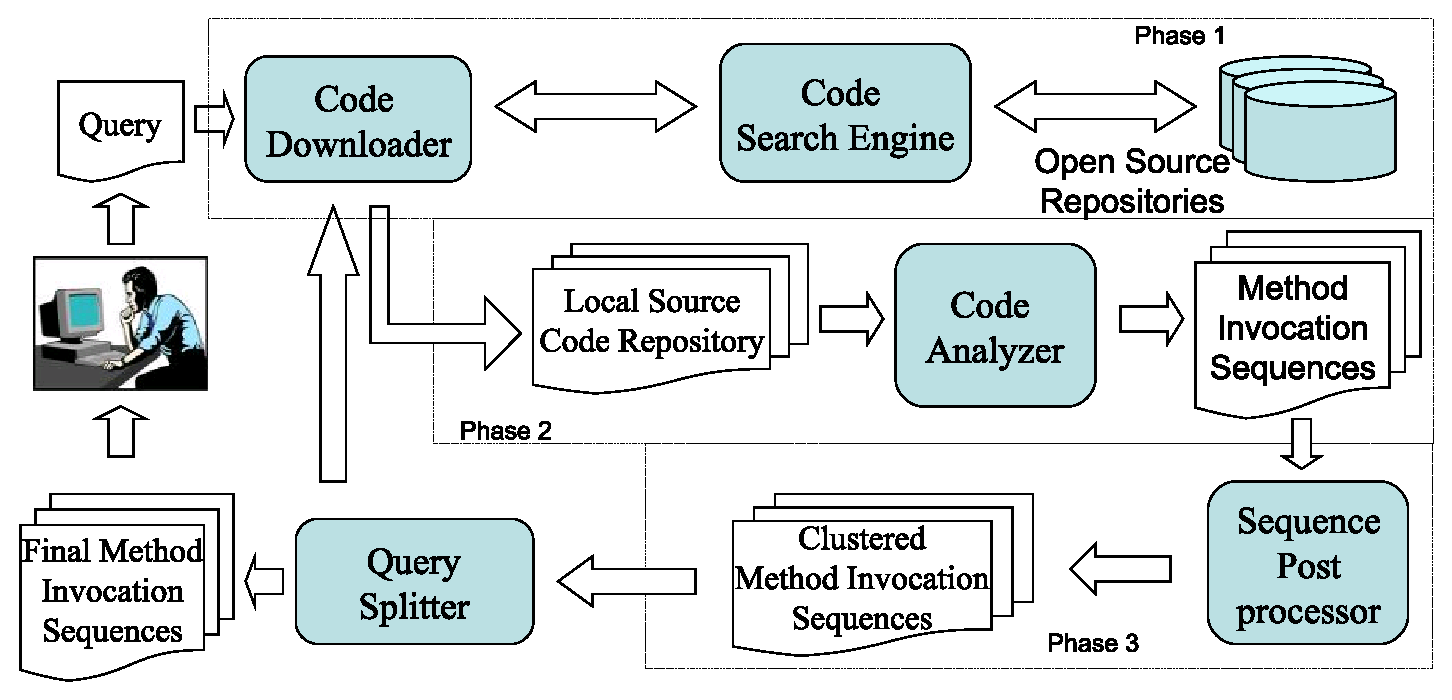
\includegraphics[scale=0.32,clip]{PARSEWeb_overview_new.eps}\vspace*{-1ex}
\caption{Overview of PARSEWeb} \label{fig:architecture}
\vspace*{-2ex}
\end{figure}
%-------------------------------------------------------------------------
\subsection{Code Search Engine}

On the web, there are a variety of
CSEs\footnote{\url{http://gonzui.sourceforge.net/links.html}}
available to assist programmers in searching for relevant code
samples like Google~\cite{GCSE} and Koders~\cite{KODERS}\Comment{,
and Krugle~\cite{KRUGLE}}. The main reason for using CSEs in our
approach is that many new frameworks or libraries emerge from day to
day and it is not practical for our own approach to maintain a
repository of all the available frameworks or libraries, and extract
results of given queries from that repository. Therefore, our
approach uses CSEs as an alternative to search in the available open
source frameworks or libraries on the web and gathers the relevant
code samples on demand. Moreover, our idea of gathering code samples
on demand makes our approach independent of any specific set of
frameworks or libraries.

In our approach, we used GCSE~\cite{GCSE} for collecting relevant code samples for the
given query, partly because GCSE provides convenient open APIs for the
third-party tools to interact with and it has been consistently
improved and maintained. However, our approach is independent of the
underlying CSE and can be extended easily to any other CSE.

%-------------------------------------------------------------------------
\subsection{Code Downloader}

The code downloader component accepts queries of the form
``\emph{Source} $\rightarrow$ \emph{Destination}'' from the
programmer and constructs a request for a CSE. The constructed
request contains both \emph{Source} and \emph{Destination} object
types. The code downloader component submits the constructed request
to CSE and downloads code samples returned by CSE to form a local
source code repository. The code samples stored in the local source
code repository are often partial and not compilable, because the
code downloader downloads only individual source files with usages
of the given \emph{Source} and \emph{Destination} object types,
instead of entire projects.
%-------------------------------------------------------------------------
\subsection{Code Analyzer}
The code analyzer component takes code samples stored in the local
source code repository as input and analyzes them to extract MISs
that can serve as solutions for the given query of the form
``\emph{Source} $\rightarrow$ \emph{Destination}''.

As code samples (i.e., source files) stored in the local source code
repository are often partial and not compilable, our approach converts
each code sample into an intermediate form. We developed the
following graph-based 
 in the conversion process to support
method inlining and to preserve control-flow information in the
intermediate form.

Initially, the code analyzer creates an Abstract Syntax Tree (AST)
for each code sample. The code analyzer uses the created AST to
build a Directed Acyclic Graph (DAG). A node in the constructed DAG
contains a single statement and an edge represents the control flow
between the two statements. The primary advantage of DAG is that DAG
supports control-flow information through branches and joins, and
provides an effective mechanism for identifying paths between any
two nodes in the graph. The statements inside loops like
\emph{while} and \emph{for} may be executed either several times or
zero time. Considering these statements once can help generate the
MIS associated with the loop. Therefore, our approach treats the
statements inside loops like \emph{while} and \emph{for} as a group
of statements that are executed either once or not. While
constructing DAG, the code analyzer performs method inlining by
replacing the method invocations of the class under analysis with
the body of the corresponding method declarations. Our approach
cannot perform method inlining if the corresponding method
declaration is \emph{abstract}. This method inlining process helps
to identify MISs that are split among methods of the class under
analysis (shown in Section~\ref{sec:parsewebtech}). If the current
class does not contain the method declaration of a method invocation
whose receiver type is \CodeIn{this} (either explicitly or
implicitly stated at the call site), the code analyzer assumes that
this method belongs to the parent class and associates a special
context called parent context (Section~\ref{sec:parentcontext}) with
that node. When needed, the code analyzer can use this parent
context for identifying the \emph{Source} object type.

The nodes in the constructed DAG contain only those statements that
result in a transformation from one object type to another. In
particular, the statements that are included in the intermediate
form belong to one of the types described below:

\begin{Itemize}
\Item Method Invocation: Generally, a method invocation with a
non-void return type can be considered as a statement that
transforms either the receiver type \Comment{(for a non-static method
invocation)} or argument types to the return type. For example, the
method invocation \CodeIn{ReturnObj obj1 = RefObj.method(Arg1,
Arg2)} can be considered as a statement that transforms objects of
type \CodeIn{RefObj}, \CodeIn{Arg1} or \CodeIn{Arg2} to
\CodeIn{ReturnObj}.
%
\Item Constructor: As a constructor generally takes some arguments,
it can be considered as a statement that transforms objects of its
argument types to the newly created object type.
%
\Item Typecast: A typecast can be considered as a transformation
statement, because it performs an explicit transformation from one
object type to another.
\end{Itemize}

Along with identifying the preceding statement types, our
approach uses several heuristics (Section ~\ref{sec:heuristics}) to
gather additional type information for each statement and this
additional type information is associated with the corresponding
node in the graph. For example, the additional type information for
method-invocation statements include the receiver object type, the
return object type, and argument types. When any of receiver, return,
or argument types matches with the given \emph{Source} object type,
the code analyzer marks the corresponding node as a \emph{Source}
node. When the return type of any statement matches with the
required \emph{Destination} type, the code analyzer marks the
corresponding node as a \emph{Destination} node.

The code analyzer extracts a MIS from the DAG by calculating the
shortest path from a \emph{Source} node to a \emph{Destination}
node. The shortest path is sufficient as every path from
\emph{Source} to \emph{Destination} nodes contain a desired
method-invocation sequence. Once a possible sequence is identified
from the DAG, the minimization process of the code analyzer extracts
a minimal MIS from the possible sequence by eliminating the extra
method invocations that are not related to the given query. This
minimal MIS is identified by traversing the sequence in the reverse
direction from the \emph{Destination} node to the \emph{Source} node
by continuously matching the receiver type and argument types of
each statement with the return type of the preceding statements. For
example, consider a possible sequence for the query
``\CodeIn{IEditorPart} $\rightarrow$ \CodeIn{ICompilationUnit}''
(where each statement consists of the receiver type, method
name, arguments, and return type):

\begin{CodeOut}
\begin{alltt}
01:IEditorPart,getEditorInput() : IEditorInput
02:CONSTRUCTOR,Shell() : Shell
03:Shell,setText(String) : void
04:JavaUI,getWorkingCopyManager() : IWorkingCopyManager
05:IWorkingCopyManager,connect(IEditorInput) : void
06:IWorkingCopyManager,getWorkingCopy(IEditorInput)
\hspace*{0.5in}: ICompilationUnit
\end{alltt}
\end{CodeOut}

The minimization process maintains a special set called a look-up set
that initially contains only the required \emph{Destination} object.
For the given possible sequence, the process starts from Statement 6
and adds the receiver type \CodeIn{IWorkingCopyManager} and the
argument type \CodeIn{IEditorInput} to the look-up set, and removes
\CodeIn{ICompilationUnit} from the look-up set. The minimization
process retains Statement 5 in the minimal MIS as its receiver type
matches with one of the types in the look-up set. In Statement 4,
the minimization process adds \CodeIn{JavaUI} to the look-up set and
removes \CodeIn{IWorkingCopyManager}. The process ignores Statements
3 and 2 as none of its object types match with the object types in
the look-up set. The minimization process ends with Statement 1 and
generates the minimal MIS as ``1,4,5,6''. These minimal MISs are
given as input to the sequence postprocessor component
(Section~\ref{sec:miner}).
%--------------------------------------------------------------------------
\subsubsection{Type Resolution}
\label{sec:heuristics}

Heuristics play a major role in the static analysis phase of our
approach. As the downloaded code samples are often partial and not
compilable, our approach relies on these heuristics to gather
information like the receiver object type, argument types, and the
return object type of each method invocation. Our approach uses five
heuristics for identifying the receiver object type and argument
types, and uses ten heuristics for identifying the return object
type. Our heuristics are based on simple language semantics like
object types of left and right hand expressions of an assignment
statement are either same or related to each other through
inheritance. Due to space limit, we explain only two of our
major heuristics used for identifying the return type of a method
invocation.

\textbf{Type Heuristic 1:} \emph{The return type of a
method-invocation statement contained in an initialization
expression is the same as the type of the declared variable.}

Consider the code sample shown below:
\begin{CodeOut}
\begin{alltt}
QueueConnection connect; QueueSession session =
\hspace*{0.4in}connect.createQueueSession(false,int)
\end{alltt}
\end{CodeOut}

%\vspace{1ex}
The receiver type of the method
\CodeIn{createQueueSession} is the type of \CodeIn{connect}
variable. Therefore, the receiver type can be simply inferred by
looking at the declaration of the \CodeIn{connect} variable. But as
our approach mainly deals with code that is partial and not
compilable, it is difficult to get the return type of the
method-invocation  \CodeIn{createQueueSession}. The reason is the
lack of access to method declarations. However, the return type can
be inferred from the type of variable \CodeIn{session} on the left
hand side of the assignment statement. As the type of variable
\CodeIn{session} is \CodeIn{QueueSession}, we can infer that the
return type of the method-invocation \CodeIn{createQueueSession} is
\CodeIn{QueueSession}.

\textbf{Type Heuristic 2:} \emph{The return type of an outermost
method-invocation contained in a return statement is the same as the
return type of the enclosing method declaration.}

Consider code sample presented below:
\begin{CodeOut}
\begin{alltt}
\textbf{public} QueueSession test()\hspace*{0.2in}\{ ...
\hspace*{0.4in}\textbf{return} connect.createQueueSession(false,int);\}
\end{alltt}
\end{CodeOut}

In this code sample, the method-invocation statement\\
\CodeIn{createQueueSession} is a part of the return statement of the
method declaration. In this scenario, we can infer the return type of
this method-invocation from the return type of the method \CodeIn{test}.
As the method \CodeIn{test} returns \CodeIn{QueueSession}, we
can infer that the return type of the
method-invocation \CodeIn{createQueueSession} is also
\CodeIn{QueueSession}.

%-------------------------------------------------------------------------
\subsubsection{Parent Context}
\label{sec:parentcontext}
A parent context includes the parent object type, if any, and
interfaces implemented by the class in the given code sample. In some of the code
samples, we observed that the \emph{Source} object type is not
explicitly available in the code sample but is described as a
parent class. The code analyzer component handles this aspect by identifying the
parent context as possible \emph{Source} object types. Consider the
query ``\CodeIn{TextEditorAction} $\rightarrow$
\CodeIn{ITextSelection}'' and a related code sample shown below:\vspace*{-2ex}

\begin{CodeOut}
\begin{alltt}
01:public class OpenAction extends TextEditorAction \{
02:\hspace*{0.1in}public void run() \{
03:\hspace*{0.3in}ITextEditor editor = getTextEditor();
04:\hspace*{0.3in}ISelectionProvider provider =
   \hspace*{0.6in}editor.getSelectionProvider();
05:\hspace*{0.3in}ITextSelection textSelection = (ITextSelection)
   \hspace*{0.6in}provider.getSelection(); \hspace*{0.1in}\}\hspace*{0.1in}\}
\end{alltt}
\end{CodeOut}

In the preceding sample, class \CodeIn{OpenAction} declares only a
\CodeIn{run} method. Although the code sample includes a solution
for the given query, it is not explicitly available as the method
declaration of \CodeIn{getTextEditor} is not available. In this
case, we can consider that the method \CodeIn{getTextEditor} is
defined in either \CodeIn{TextEditorAction} or its parent classes.
Therefore, class \CodeIn{TextEditorAction} can be considered as
receiver type for the method \CodeIn{getTextEditor}. With this consideration, our approach can
identify that this code sample is a possible solution for the given
query.
%--------------------------------------------------------------------------
\subsection{Sequence Postprocessor}
\label{sec:miner} The sequence postprocessor component clusters similar MISs
and ranks the clustered MISs. Clustering of MISs helps to identify
distinct possible MISs and also reduces the total number of MISs.
This reduction of the number of results can help programmers quickly
identify the desired MIS for the given query. To further assist
programmers, the sequence postprocessor also sorts the clustered results.
These sorted results can help programmers identify sequences that
are more frequently used for addressing the given query.

\subsubsection{Sequence Clustering}
\label{sec:rankingCriteria}

\Comment{We observed that queries often result in similar MISs. To cluster
these similar MISs, }We next describe the heuristic used
by our approach for identifying and clustering similar MISs.
To identify similar MISs, our approach ignores the order of statements in the
extracted MISs. Our approach considers MISs with the same set of
statements and with a different order as similar.
For example, consider MISs ``2,3,4,5'' and ``2,4,3,5'' where each
number indicates a single statement associated with the node
in the constructed DAG. Our approach considers
these sequences as similar because different programmers
may write intermediate statements in different orders and these
statements may be independent from one another.

To further cluster the identified MISs, 
our approach identifies MISs with minor differences and
clusters those identified MISs. We introduce an attribute,
called \emph{cluster precision}, which defines the number of statements by
which two given MISs differ each other. This attribute is
configurable and helps the sequence postprocessor in further 
clustering the identified MISs. Our approach considers
MISs that differ by the given \emph{cluster precision} value
as similar, irrespective of the order of statements in
those MISs. For example, consider MISs ``8,9,6,7'' and ``8,6,10,7''. These two
sequences have three common statements (8,6,7) and differ by a
single statement. Our approach considers these two MISs as similar
under a \emph{cluster precision value} of one, as both the sequences
differ by only one method invocation. This heuristic is based on the
observation that different MISs in the final set of sequences often
contain overloaded forms of the same method invocation.
%-------------------------------------------------------------------------
\subsubsection{Sequence Ranking}
\label{sec:rankingCriteria}

In general, many queries result in more than one possible solution,
and not all solutions are of the same importance to the programmer.
To assist the programmer in quickly identifying the desired MISs,
our approach uses two ranking heuristics and sorts the final
set of MISs.

\textbf{Ranking Heuristic 1:} \emph{Higher the frequency
$\rightarrow$ Higher the rank}

This heuristic is based on the observation that more-used MISs might
be more likely to be used compared to less-used MISs. Therefore,
MISs with higher frequencies are given a higher preference.

\textbf{Ranking Heuristic 2:} \emph{Shorter the length $\rightarrow$
Higher the rank}

This ranking heuristic, which was originally proposed in the
Prospector~\cite{prospector:jungloid} approach, is based on the
length of the MIS. Shorter sequences are given a higher preference to
longer sequences. This heuristic is considered based on the
observation that programmers would often tend to use shorter
sequences instead of longer ones to achieve their task.

%-------------------------------------------------------------------------
\subsection{Query Splitter}
\label{sec:querysplitter}
Query splitting is an additional heuristic used by our approach to
address the problem of lack of code samples in the results of CSE.
We observed that a code sample for some of the queries is split
among different files instead of having the entire sample in the
same file. The query splitting heuristic helps to address this
problem by splitting the given query into multiple sub-queries. The
algorithm of our approach including the query splitting heuristic is
described in Algorithm ~\ref{alg:parsewebalgo}.

Initially, our approach accepts the query of the form
``\emph{Source} $\rightarrow$ \emph{Destination}'' and tries to
suggest solutions. If no possible MISs are found, our approach tries
to infer the immediate alternate destinations (\emph{AltDest}) by
constructing a new query that includes only the \emph{Destination}
object type. A query with just the \emph{Destination} object
type provides different possible MISs, referred as
\emph{DestOnlyMISs}, that result in the object of the
\emph{Destination} type. In these \emph{DestOnlyMISs}, the
\emph{Source} can be of any object type. Our approach infers the
\emph{AltDestSet} by identifying the receiver type and argument
types in the last method invocation (\emph{lastMI}) of each MIS in
the \emph{DestOnlyMISs} set. The primitive types, such as
\CodeIn{int}, are ignored while identifying the \emph{AltDest}. For
each of the \emph{AltDest}, new MISs are generated by constructing
queries of the form ``\emph{Source} $\rightarrow$ \emph{AltDest}''.
The \emph{lastMI} of the earlier sequence is appended to the new set
of sequences to generate a complete MIS. In case our approach
including the query splitting is not able to suggest any MISs, we
simply return the \emph{DestOnlyMISs}.

\begin{algorithm}[t]
\begin{CodeOut}
\SetLine
\KwIn{Source and Destination object types}
\KwOut{Method-Invocation Sequences}
Extract $MISs$ for the Query ``Source$\rightarrow$Destination''\;
\If{$MISs$ are not empty}{\Return MISs\;}
//Query Splitting\\
Extract $DestOnlyMISs$ for the Query ``Destination''\;
\For{$MIS$ in $DestOnlyMISs$}{
$lastMI$ = $MIS$.lastMethodInvocation()\;
$AltDestSet$ = $ReceiverType$ and $ArgTypes$ of $lastMI$\;
Intialize $FinalMISs$\;
\For{$AltDest$ in $AltDestSet$}{
Extract $AltMIS$ for the Query ``Source$\rightarrow$AltDest''\;
Append $lastMI$ to $AltMIS$\;
Add $AltMIS$ to $FinalMISs$\;
}}
\If{$FinalMISs$ are not empty}{
\Return $FinalMISs$
}\Else{\Return $DestOnlyMISs$\;}
\end{CodeOut}
\caption{Pseudocode of the PARSEWeb algorithm with the query
splitting heuristic} \label{alg:parsewebalgo}
\end{algorithm}